\documentclass[bachelor, och, otchet]{../SCWorks}
% Тип обучения (одно из значений):
%    bachelor   - бакалавриат (по умолчанию)
%    spec       - специальность
%    master     - магистратура
% Форма обучения (одно из значений):
%    och        - очное (по умолчанию)
%    zaoch      - заочное
% Тип работы (одно из значений):
%    coursework - курсовая работа (по умолчанию)
%    referat    - реферат
%  * otchet     - универсальный отчет
%  * nirjournal - журнал НИР
%  * digital    - итоговая работа для цифровой кафедры
%    diploma    - дипломная работа
%    pract      - отчет о научно-исследовательской работе
%    autoref    - автореферат выпускной работы
%    assignment - задание на выпускную квалификационную работу
%    review     - отзыв руководителя
%    critique   - рецензия на выпускную работу

% * Добавлены вручную. За вопросами к @mchernigin
\usepackage{../preamble}

\begin{document}

% Кафедра (в родительном падеже)
\chair{информатики и программирования}

% Тема работы
\title{Машинно"=зависимые языки программмирования. Лабораторная работа №3}

% Курс
\course{2}

% Группа
\group{251}

% Факультет (в родительном падеже) (по умолчанию "факультета КНиИТ")
\department{факультета компьютерных наук и информационных технологий}

% Специальность/направление код - наименование
% \napravlenie{02.03.02 "--- Фундаментальная информатика и информационные технологии}
% \napravlenie{02.03.01 "--- Математическое обеспечение и администрирование информационных систем}
% \napravlenie{09.03.01 "--- Информатика и вычислительная техника}
\napravlenie{09.03.04 "--- Программная инженерия}
% \napravlenie{10.05.01 "--- Компьютерная безопасность}

% Для студентки. Для работы студента следующая команда не нужна.
\studenttitle{студентки}

% Фамилия, имя, отчество в родительном падеже
\author{Потапкиной Маргариты Андреевны}

% Заведующий кафедрой 
\chtitle{доцент, к.\,ф.-м.\,н.}
\chname{С.\,В.\,Миронов}

% Руководитель ДПП ПП для цифровой кафедры (перекрывает заведующего кафедры)
% \chpretitle{
%     заведующий кафедрой математических основ информатики и олимпиадного\\
%     программирования на базе МАОУ <<Ф"=Т лицей №1>>
% }
% \chtitle{г. Саратов, к.\,ф.-м.\,н., доцент}
% \chname{Кондратова\, Ю.\,Н.}

% Научный руководитель (для реферата преподаватель проверяющий работу)
\satitle{старший преподаватель} %должность, степень, звание
\saname{Е.\,М.\,Черноусова}

% Руководитель практики от организации (руководитель для цифровой кафедры)
\patitle{доцент, к.\,ф.-м.\,н.}
\paname{С.\,В.\,Миронов}

% Руководитель НИР
\nirtitle{доцент, к.\,п.\,н.} % степень, звание
\nirname{В.\,А.\,Векслер}

% Семестр (только для практики, для остальных типов работ не используется)
\term{2}

% Наименование практики (только для практики, для остальных типов работ не
% используется)
\practtype{учебная}

% Продолжительность практики (количество недель) (только для практики, для
% остальных типов работ не используется)
\duration{2}

% Даты начала и окончания практики (только для практики, для остальных типов
% работ не используется)
\practStart{01.07.2024}
\practFinish{13.01.2024}

% Год выполнения отчета
\date{2025}

\maketitle

% Включение нумерации рисунков, формул и таблиц по разделам (по умолчанию -
% нумерация сквозная) (допускается оба вида нумерации)
\secNumbering

\tableofcontents

% Раздел "Обозначения и сокращения". Может отсутствовать в работе
% \abbreviations
% \begin{description}
%     \item ... "--- ...
%     \item ... "--- ...
% \end{description}

% Раздел "Определения". Может отсутствовать в работе
% \definitions

% Раздел "Определения, обозначения и сокращения". Может отсутствовать в работе.
% Если присутствует, то заменяет собой разделы "Обозначения и сокращения" и
% "Определения"
% \defabbr

\section{Текст задания}
\input{task.txt}

\section{Тексты программ на языке ассемблера с комментариями}
\subsection{Программа 1}
\small
\inputminted{nasm}{1.asm}
\normalsize
\subsection{Программа 2}
\small
\inputminted{nasm}{2.asm}
\normalsize

\section{Скриншоты запуска программ}
\begin{figure}[H]
\centering
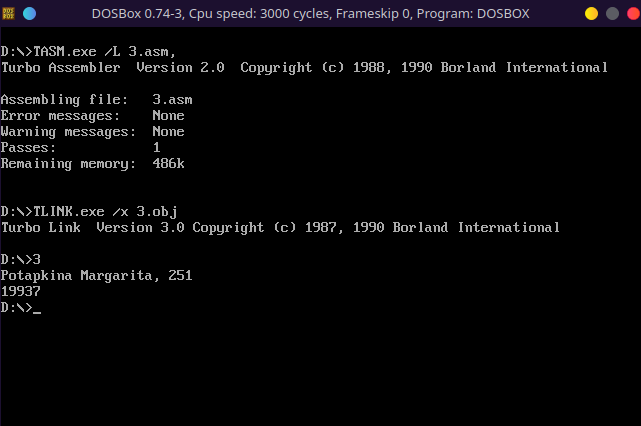
\includegraphics[scale=0.9]{1.png}
\caption {Скриншот запуска программы 1}
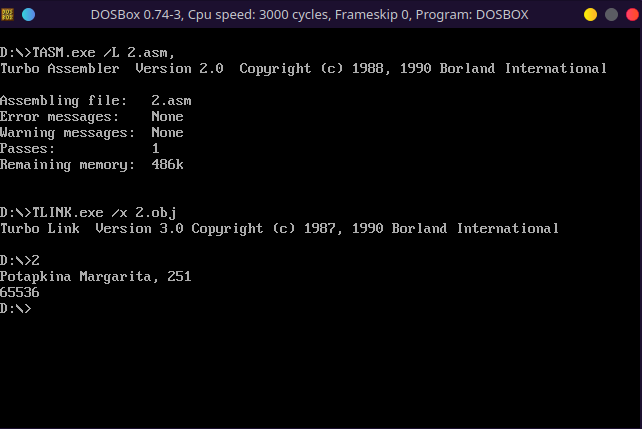
\includegraphics[scale=0.9]{2.png}
\caption {Скриншот запуска программы 2}
\end{figure}

\section{Ответы на контрольные вопросы}
\begin{enumerate}
\item Чем отличается деление на байт от деления на слово? (где должно располагаться делимое, куда попадут частное от деления и остаток от деления)

При делении на байт делимое должно располагаться в регистре AX, частное попадёт в регистр AL, а остаток "--- в регистр AH.

При делении на слово делимое располагается в паре регистров [DX, AX] (регистр DX содержит старшую значимую часть, а регистр AX "--- младшую), частное попадает в регистр AX, а остаток "--- в регистр DX.
\item Каков механизм действия команды cmp? В паре с какими командами она обычно используется?

CMP выполняет сравнение двух операндов, вычитая второй из первого, результат она не сохраняет, а лишь обновляет флаги состояния в соответствии с ответом. Основное назначение этой команды "--- организация условных переходов. Она используется в паре с командами условного перехода: для арифметического сравнения со знаком это JL (<), JLE ($\leq$), JG (>) и JGE ($\geq$), для сравнения без знака "--- JB (<), JBE ($\leq$), JA (>) и JAE ($\geq$), а также JE (=) и JNE ($\ne$).

\item На какие флаги реагируют команды условного перехода для чисел со знаком и для чисел без знака?

Команды условного перехода для чисел со знаком реагируют на флаги знака (SF), переполнения (OF) и нуля (ZF). Для чисел без знака учитываются флаг переноса (CF, показывает, какое из чисел больше) и флаг нуля (ZF, определяет равенство).

\item С помощью команд условного и безусловного перехода выполните программную реализацию алгоритма ветвления для определения наименьшего числа из двух заданных. Алгоритм изображен в виде блок"=схемы, приведенной на рис. 4.1.

\begin{figure}[H]
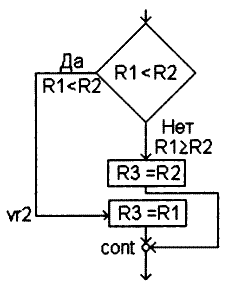
\includegraphics{block-scheme.png}
\caption{Организация ветвления на машинном уровне: \newline
R1 "--- первое число хранится в регистре AX; \newline
R2 "--- второе число хранится в регистре BX; \newline
R3 "--- результат заносится в регистр DX; \newline
vr2, cont "--- метки команд. \newline}
\end{figure}

\inputminted{nasm}{example.asm}

\item Каков механизм работы команды организации цикла LOOP?

Команда LOOP в конце каждой итерации уменьшает значение регистра CX на 1 и передаёт управление на указанную в команде метку, если CX не стал равен нулю. Если же декремент CX привёл к получению в нём 0, то цикл завершается, и выполняется следующая за циклом команда.

\item Как с помощью команды сдвига можно умножить знаковое число, хранящееся в АХ, на 2 в n"=ой степени? 

Необходимо применить команду арифметического (для того, чтобы сохранить знак числа) сдвига влево (SAL) на n. Команда будет выглядеть следующим образом: SAL AX,n (до этого нужно инициализовать переменную n, например, так: n EQU <число>).

\item Как с помощью команды сдвига проверить содержимое регистра ВХ на четность?

Необходимо выполнить сдвиг вправо (SHR) на 1. При этом младший бит попадёт во флаг переноса (CF). Дальше можно применить команду JC для нечётных чисел (произойдёт переход, только если флаг переноса выставлен в 1, т.е. младший бит был равен 1, т.е. число было нечётным), а команду JNC "--- для чётных.

\end{enumerate}
% Отобразить все источники. Даже те, на которые нет ссылок.
% \nocite{*}

% Окончание основного документа и начало приложений Каждая последующая секция
% документа будет являться приложением
\appendix
\end{document}
